% Options for packages loaded elsewhere
\PassOptionsToPackage{unicode}{hyperref}
\PassOptionsToPackage{hyphens}{url}
%
\documentclass[
]{article}
\usepackage{lmodern}
\usepackage{amssymb,amsmath}
\usepackage{ifxetex,ifluatex}
\ifnum 0\ifxetex 1\fi\ifluatex 1\fi=0 % if pdftex
  \usepackage[T1]{fontenc}
  \usepackage[utf8]{inputenc}
  \usepackage{textcomp} % provide euro and other symbols
\else % if luatex or xetex
  \usepackage{unicode-math}
  \defaultfontfeatures{Scale=MatchLowercase}
  \defaultfontfeatures[\rmfamily]{Ligatures=TeX,Scale=1}
\fi
% Use upquote if available, for straight quotes in verbatim environments
\IfFileExists{upquote.sty}{\usepackage{upquote}}{}
\IfFileExists{microtype.sty}{% use microtype if available
  \usepackage[]{microtype}
  \UseMicrotypeSet[protrusion]{basicmath} % disable protrusion for tt fonts
}{}
\makeatletter
\@ifundefined{KOMAClassName}{% if non-KOMA class
  \IfFileExists{parskip.sty}{%
    \usepackage{parskip}
  }{% else
    \setlength{\parindent}{0pt}
    \setlength{\parskip}{6pt plus 2pt minus 1pt}}
}{% if KOMA class
  \KOMAoptions{parskip=half}}
\makeatother
\usepackage{xcolor}
\IfFileExists{xurl.sty}{\usepackage{xurl}}{} % add URL line breaks if available
\IfFileExists{bookmark.sty}{\usepackage{bookmark}}{\usepackage{hyperref}}
\hypersetup{
  hidelinks,
  pdfcreator={LaTeX via pandoc}}
\urlstyle{same} % disable monospaced font for URLs
\usepackage{graphicx}
\makeatletter
\def\maxwidth{\ifdim\Gin@nat@width>\linewidth\linewidth\else\Gin@nat@width\fi}
\def\maxheight{\ifdim\Gin@nat@height>\textheight\textheight\else\Gin@nat@height\fi}
\makeatother
% Scale images if necessary, so that they will not overflow the page
% margins by default, and it is still possible to overwrite the defaults
% using explicit options in \includegraphics[width, height, ...]{}
\setkeys{Gin}{width=\maxwidth,height=\maxheight,keepaspectratio}
% Set default figure placement to htbp
\makeatletter
\def\fps@figure{htbp}
\makeatother
\setlength{\emergencystretch}{3em} % prevent overfull lines
\providecommand{\tightlist}{%
  \setlength{\itemsep}{0pt}\setlength{\parskip}{0pt}}
\setcounter{secnumdepth}{-\maxdimen} % remove section numbering

\author{}
\date{}

\begin{document}

\textbf{Proyecto Final de seguridad y Auditoria}

\textbf{Universidad Mariano Gálvez Sede de Boca del Monte}

\textbf{David Alejandro Serrano Salazar 7690-13-19355}

\textbf{Ervin Gabriel Laferre Guevara 7690-16-10153}

\textbf{Guatemala, 06 de noviembre de 2021}

\textbf{Configuración de las maquinas asignadas:}

Cada una de las maquinas virtuales que instalamos están relacionadas con
una IP estática que se le dio por medio del PFSENSE que actuara tanto
como nuestro servidor de VPN como nuestro FIREWALL.

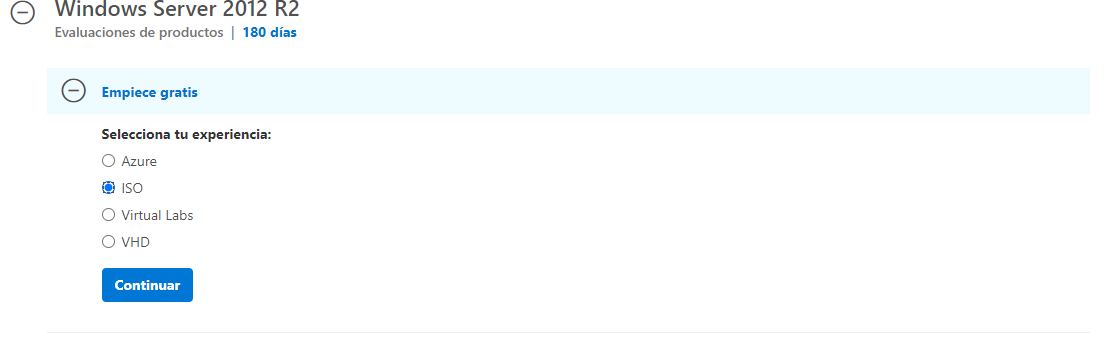
\includegraphics[width=1.71875in,height=1.13542in]{media/image1.png}

\textbf{Servidor FREEDSB}

Como vemos tiene una IP asignada por medio de nuestra VPN como su IP
local.

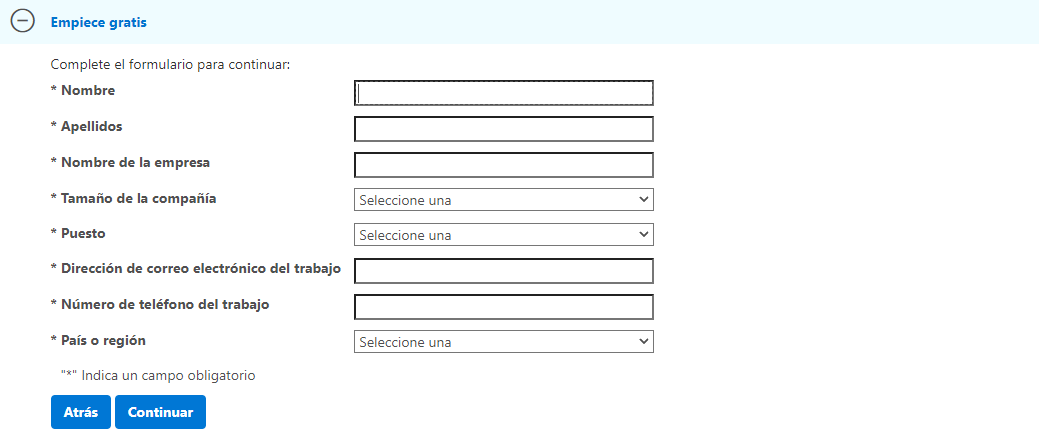
\includegraphics[width=4.5in,height=2.96875in]{media/image2.png}

\textbf{CONFIGURACION DEL FIREWALL.}

Como vemos existen varios usuarios que se crearon para tener distintos
accesos y niveles de seguridad dependiendo el tipo de usuario que
tengamos, asimismo se entablaron grupos que son administrador para que
se puedan modificar desde cualquier maquina y no solo se dependa de una
persona para realizar dicha configuración, en esta pantalla para agregar
permisos bastaría con agregar (botón verde) y la ventana que levanta
ingresar los datos requeridos y seleccionar si es administrador o no.

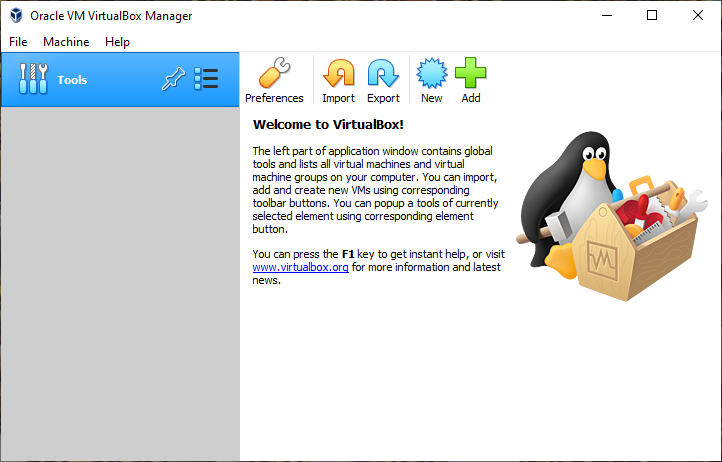
\includegraphics[width=6.1375in,height=2.91319in]{media/image3.png}

\textbf{CONFIGURACION DE REGLAS.}

Para configurar las reglas dentro del firewall nos vamos a la barra de
menú y encontraremos la parte de FIREWALL, pinchamos en ella. Y nos
desplegara una tabla con todas las reglas configuradas a cada uno de los
usuarios, donde hemos podido denegar el trafico especifico a una página,
así como a una sección de IPS para prohibir el uso de redes sociales, la
cual esta regla se puede activar a una cantidad infinita de usuario,
también hemos permitido el acceso y denegar el acceso a la pagina de la
UMG con la finalidad de probar esta.

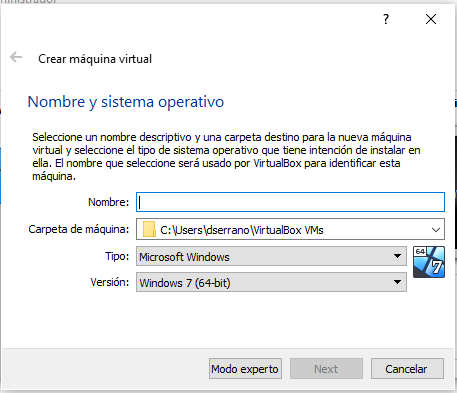
\includegraphics[width=6.38542in,height=3.21872in]{media/image4.png}

\textbf{CONFIGURACION DE IP PUBLICA}

La configuración de cada una de estas IPS es necesaria para el
funcionamiento de la VPN, con la cual, una nos servirá para la red
interna que creará la VPN y la otra nos servirá para la salida del
internet.

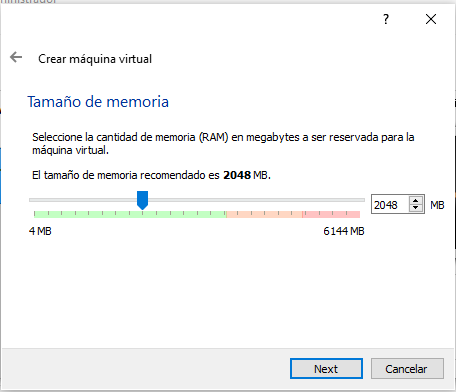
\includegraphics[width=6.1375in,height=3.09028in]{media/image5.png}

\textbf{CONFIGURACION DE IP PRIVADA}

Ya una vez dentro creamos reglas de comportamiento. Una sola regla
activa para todos lados de ida y vuelta la configuración, como puede ser
el caso del internet, o puertos específicos para conexiones, tal es el
caso de algunos servicios como Microsoft Teams, Meet, Skype entre otros.

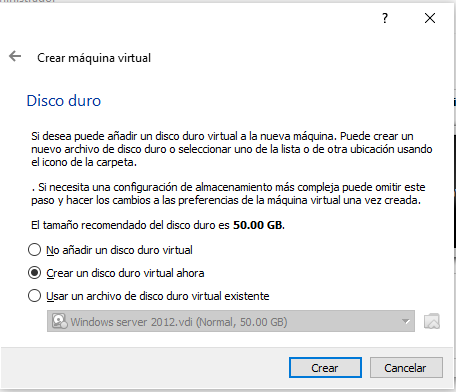
\includegraphics[width=6.04375in,height=2.82292in]{media/image6.png}

\textbf{CONFIGURACION DE IP PRIVADA}

Cada vez que realizamos una actualización del firewall sin importar la
acción que estemos realizando nos encontraremos con el siguiente
escenario al momento de darle guardar para activar las reglas nos saldrá
un mensaje de confirmación para validar que estemos de acuerdo y si lo
estamos nos saldrá el mensaje que vemos a continuación, indicando que la
reglas han sido aplicadas inmediatamente se puede visualizar en los
clientes estos cambios.

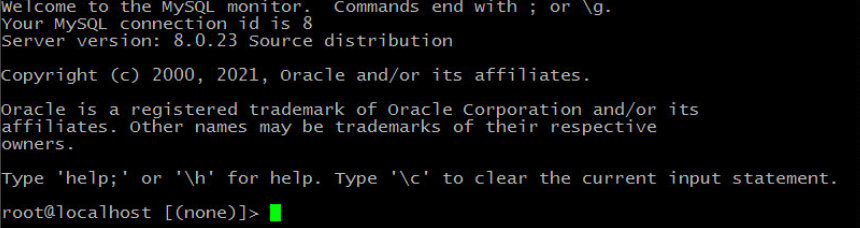
\includegraphics[width=5.67708in,height=2.35417in]{media/image7.png}

\textbf{PRUEBAS DE LAS REGLAS IMPLEMENTADAS}

Como describimos en la parte de arriba el servidor tiene la IP con
terminación 7 en las reglas del FIREWALL, indicamos que se podía enviar
paquetes ICMP, como podemos visualizar en la siguiente imagen

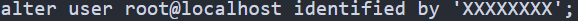
\includegraphics[width=4.9375in,height=2.28125in]{media/image8.png}

Luego de esto realizamos una actualización de esta regla activando una
restricción completa a la red que no puedan enviar este tipo de
paquetes, como vemos en la imagen continua no ha recibido ningún
paquete, todos se perdieron.

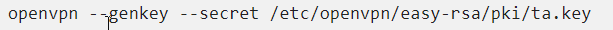
\includegraphics[width=5.29167in,height=1.92708in]{media/image9.png}

\textbf{CREACION DE REGLAS DENTRO DEL FIREWALL}

En el apartado de Firewall, existe un botón color verde que indica
agregar (ADD), en el cual nos dará una ventana donde podemos configurar
las reglas que creamos necesarias e indicar el usuario o los usuarios
que afectará esta regla, en la imagen siguiente, veremos el ejemplo de
la creación de una de estas para que la cualquier IP pueda visualizar el
SERVIDOR ADD.

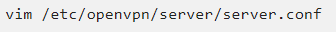
\includegraphics[width=5.95833in,height=2.75in]{media/image10.png}

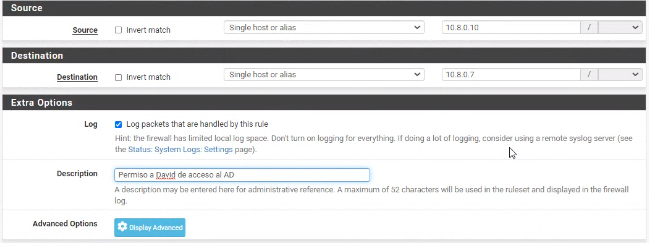
\includegraphics[width=6.1375in,height=2.29792in]{media/image11.png}

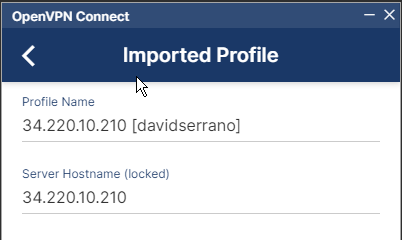
\includegraphics[width=6.1375in,height=1.19167in]{media/image12.png}

Una vez llenamos todos los campos que hemos visto en la imagen,
pinchamos en el botón de guardar, y nos regresara a la pantalla anterior
donde estarán todas las reglas listadas dentro de la tabla, está
actualmente creada aparecerá desactivada y lo único que tendríamos que
realizar es la activación de dicha regla, para que este vigente.

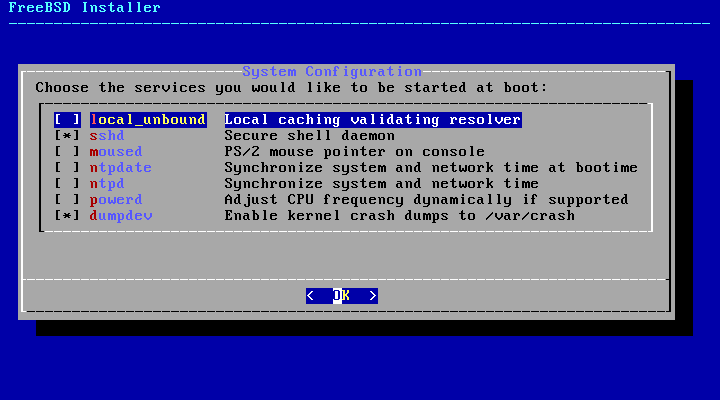
\includegraphics[width=5.98958in,height=2.58333in]{media/image13.png}

Como vimos anteriormente el mensaje de aplicar cambios nos aparecerá y
luego se activará, otro ejemplo que pudimos realizar es la restricción
de internet a la IP que se conecte en este caso bloqueamos la IP de
Google.

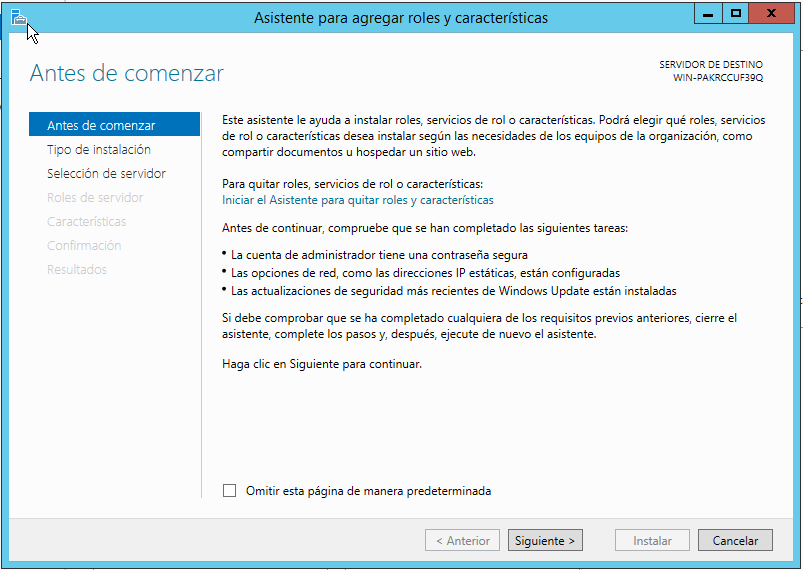
\includegraphics[width=6.13542in,height=1.5in]{media/image14.png}

Luego la desactivamos y vemos que es sencillo realizar reglas en el
firewall para limitar el acceso a internet o algún segmento especifico
de la red.

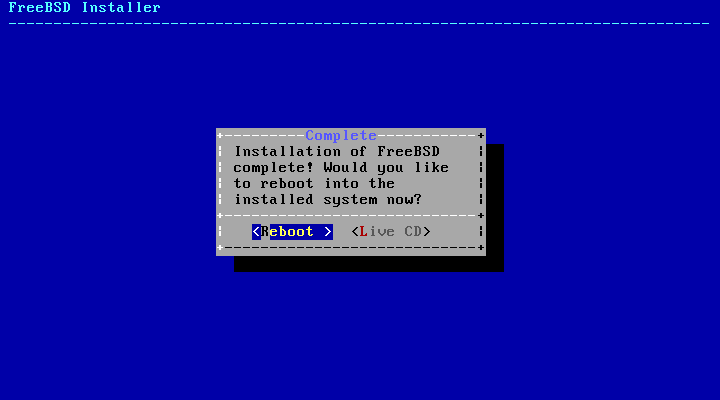
\includegraphics[width=6.11458in,height=2.09375in]{media/image15.png}

\end{document}
